
\section{Exercise 1: Resistance Measurement}

\subsection{Objective}
The objective of this exercise is to measure the resistance of a resistor using a digital multimeter and compare the measured value with the calculated value.

\subsection{Equipment}
\begin{itemize}
    \item Digital Multimeter (DMM)
    \item Resistors ($470\Omega$, $1k\Omega$, $4.3k\Omega$)
    \item Breadboard
    \item Power Supply
\end{itemize}

\newpage
\thispagestyle{plain}

\subsection{Procedure}
\begin{enumerate}
    \item We have connected each resistor to the breadboard and measured the resistance using the digital multimeter.
    \item We have calculated the each resistor value using the values according to this table:
    \begin{table}[h]
        \centering
        \begin{tabular}{|c|c|c|c|c|c|}
            \hline
            Color   & 1st Band & 2nd Band & 3rd Band & Multiplier (\(\Omega\)) & Tolerance (\%) \\ \hline
            Black   & 0        & 0        & 0        & 1                     & -              \\ \hline
            Brown   & 1        & 1        & 1        & 10                    & \(\pm\)1       \\ \hline
            Red     & 2        & 2        & 2        & 100                   & \(\pm\)2       \\ \hline
            Orange  & 3        & 3        & 3        & 1,000                 & -              \\ \hline
            Yellow  & 4        & 4        & 4        & 10,000                & -              \\ \hline
            Green   & 5        & 5        & 5        & 100,000               & \(\pm\)0.5     \\ \hline
            Blue    & 6        & 6        & 6        & 1,000,000             & \(\pm\)0.25    \\ \hline
            Violet  & 7        & 7        & 7        & 10,000,000            & \(\pm\)0.1     \\ \hline
            Gray    & 8        & 8        & 8        & 100,000,000           & \(\pm\)0.05    \\ \hline
            White   & 9        & 9        & 9        & 1,000,000,000         & -              \\ \hline
            Gold    & -        & -        & -        & 0.1                   & \(\pm\)5       \\ \hline
            Silver  & -        & -        & -        & 0.01                  & \(\pm\)10      \\ \hline
        \end{tabular}
        \caption{Resistor Color Code Table \cite{resistor-calculator}}
    \end{table}
    \begin{itemize}
        \item In order to calculate the resistance value of a resistor using the color code, we can use the following formula:
        \[\text{Resistance} = (1^{st}~\text{Band} \times 10 + 2^{nd}~\text{Band}) \times \text{Multiplier}\]
        \item These are the results of the calculations:
        \begin{table}[h]
            \centering
            \begin{tabular}{|c|c|}
                \hline
                Resistor & Color Code \\
                \hline
                \(R_1 = 470\Omega\) & Yellow-Violet-Brown \\
                \(R_2 = 1k\Omega\) & Brown-Black-Red \\
                \(R_3 = 4.3k\Omega\) & Yellow-Orange-Red \\
                \hline
            \end{tabular}
            \caption{Color Codes for Given Resistors}
        \end{table}
    \end{itemize}
    
    \newpage
    \thispagestyle{plain}
    
    \item We have measured the resistor values using the digital multimeter and these are the results:
    \begin{figure}[h]
        \centering
        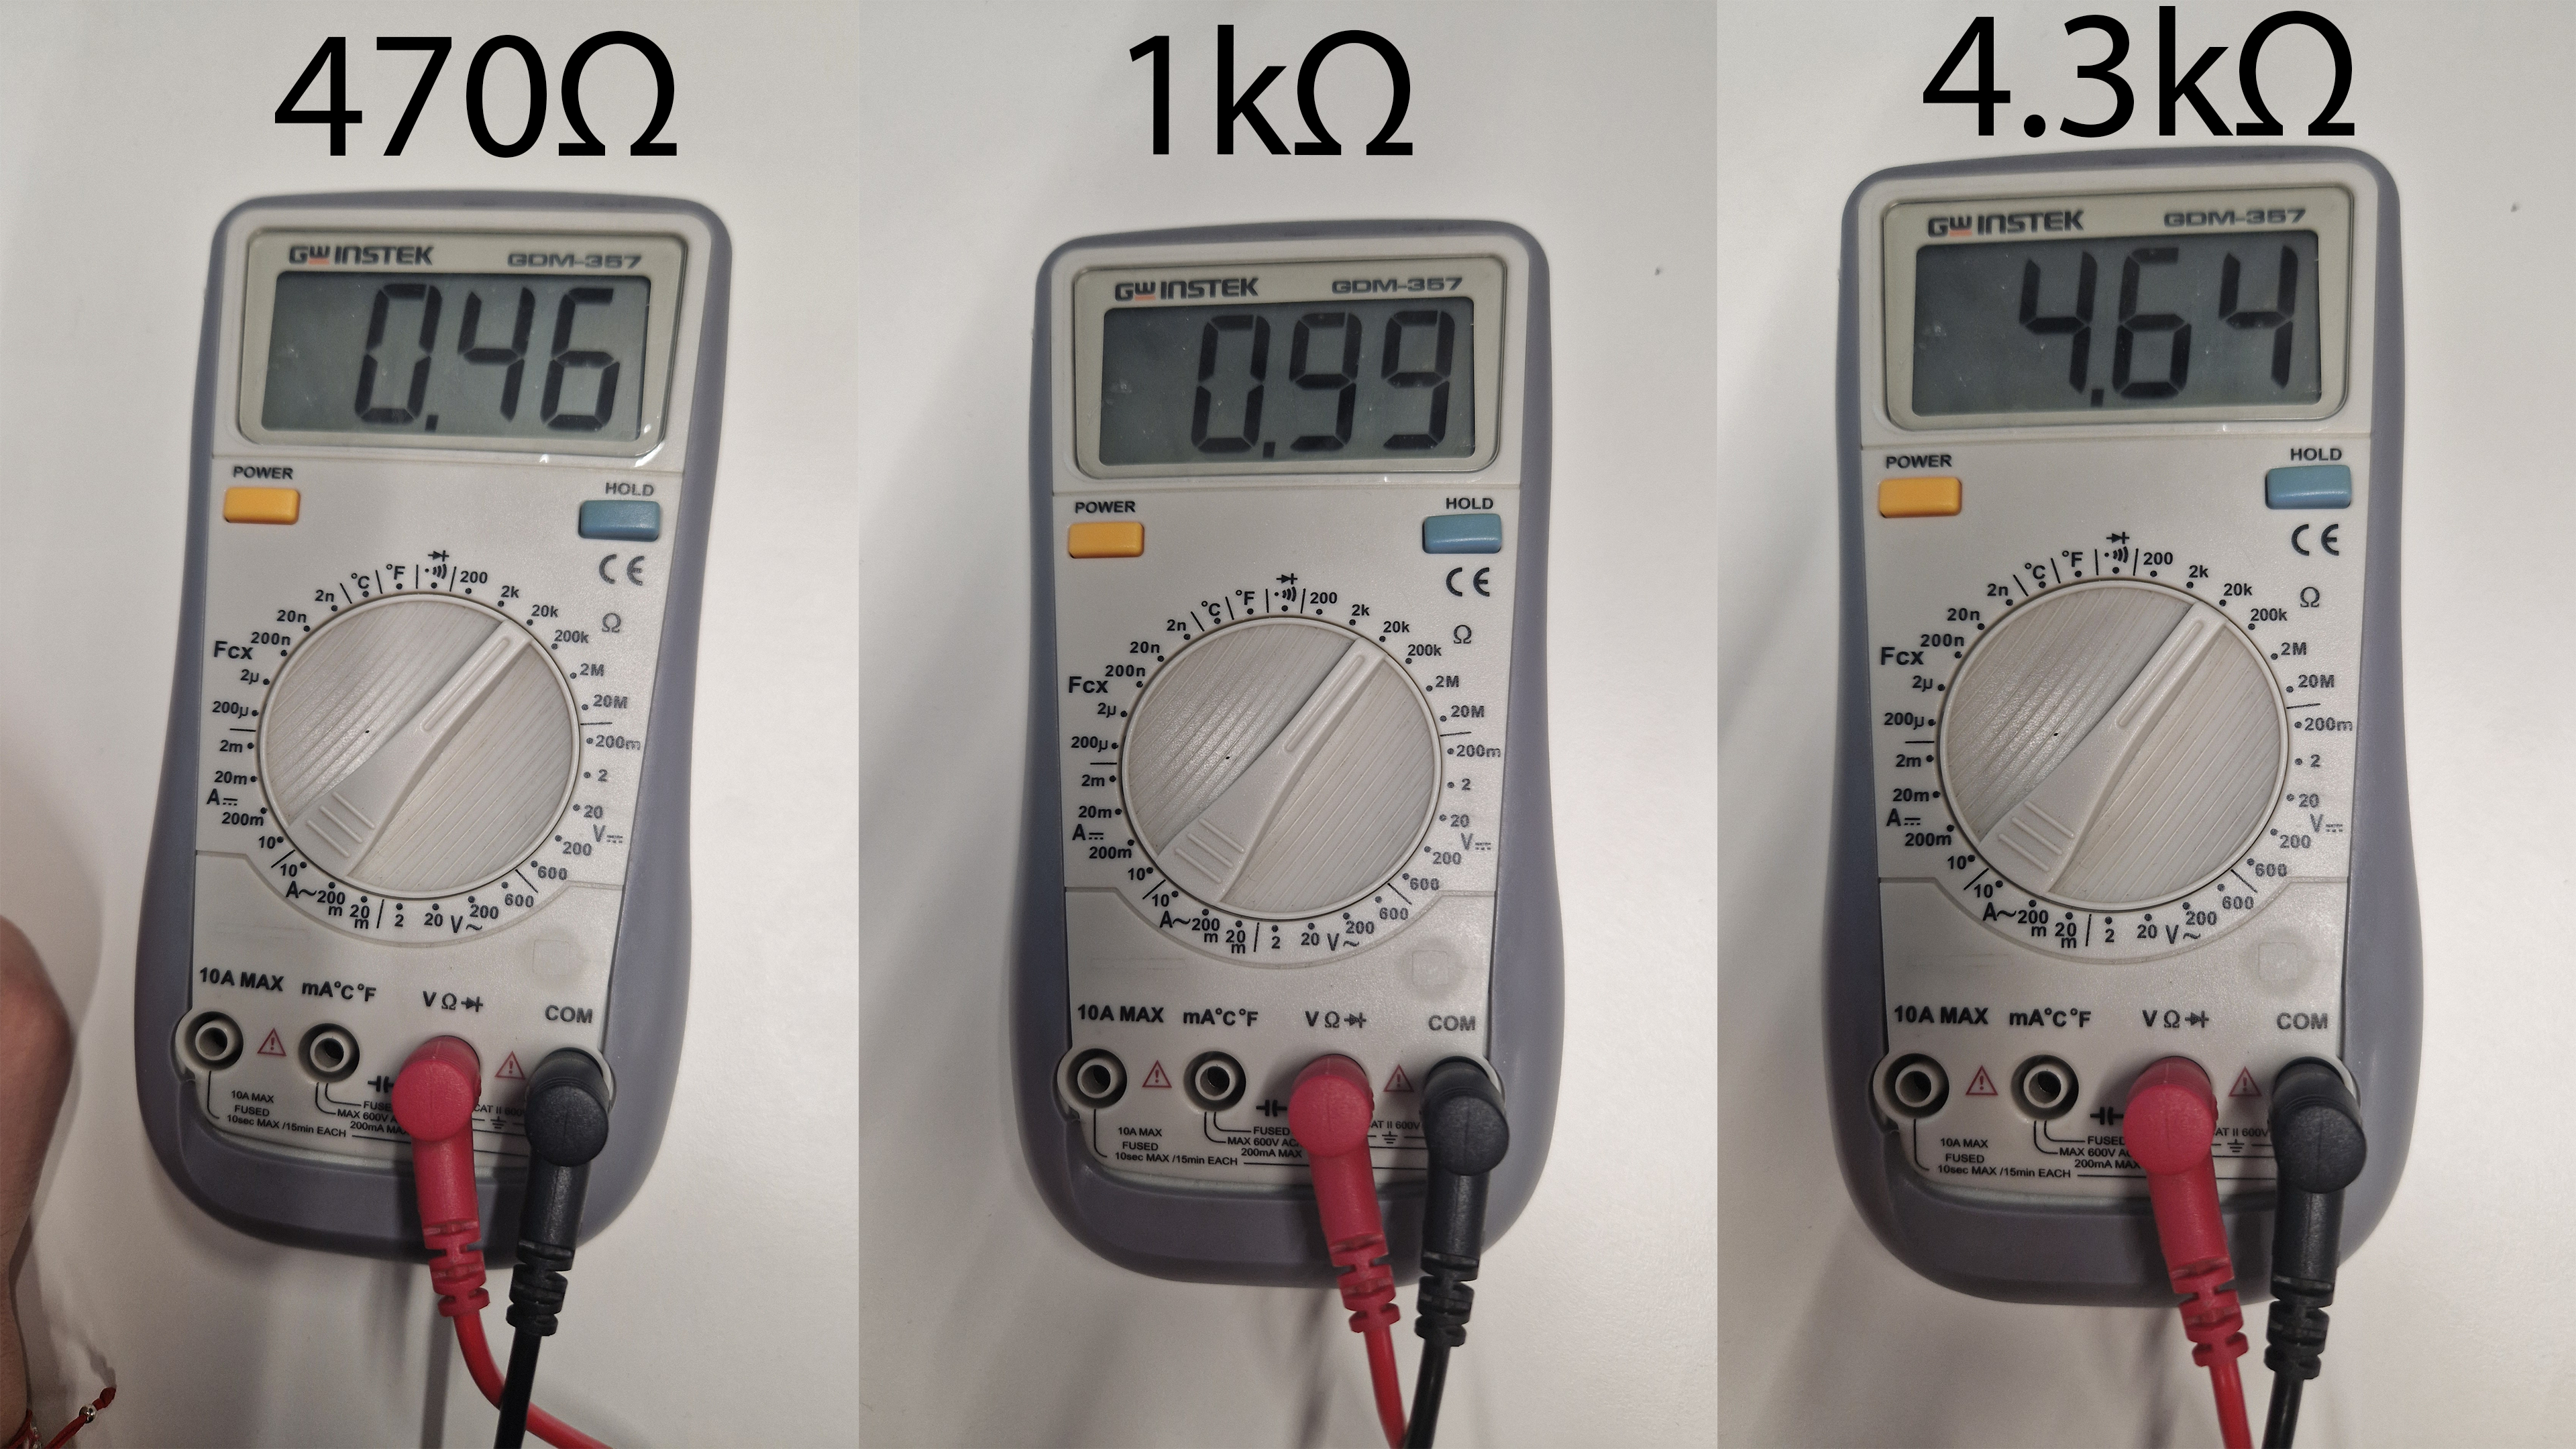
\includegraphics[width=1\textwidth]{assets/resistor-calculations.png}
        \caption{Resistor Measurements Using Digital Multimeter}
        \label{measured-resistors}
    \end{figure}
    \begin{table}[h]
        \centering
        \begin{tabular}{|c|c|c|}
            \hline
            Expected & Calculated & Color Code \\
            \hline
            \(R_1 = 470\Omega\) & \(460\Omega\) & Yellow-Violet-Brown \\
            \(R_2 = 1k\Omega\) & \(0.99k\Omega\) & Brown-Black-Red \\
            \(R_3 = 4.3k\Omega\) & \(4.64k\Omega\) & Yellow-Orange-Red \\
            \hline
        \end{tabular}
        \caption{Real Measured Values of Resistors According to the Figure\#\ref{measured-resistors}}
    \end{table}
\end{enumerate}

\subsection{Results}
We have measured the resistance of the resistors and compared the results with the expected values and the measured values are close to the calculated values. The differences between the measured and calculated values are due to the tolerance of the resistors. The tolerance of the resistors are \(\pm5\%\) and \(\pm1\%\). The measured values are within the tolerance range.

\newpage
\thispagestyle{plain}
